\documentclass[a4paper]{article}
\usepackage[letterpaper,margin=1in]{geometry}
\usepackage{blindtext}
\usepackage{lastpage}
\usepackage{fancyhdr}
\usepackage{setspace}
\usepackage{amsmath}
\usepackage{graphicx}
\usepackage{float}
\graphicspath{{C:/Users/Bilge Kutay/Downloads/}}

% Configure the header
\pagestyle{fancy} % Enable fancy headers
\fancyhead[L]{CE 591} % Left-aligned header
\fancyhead[C]{Wave Hydrodynamics} % Centered header
\fancyhead[R]{26/03/2025} % Right-aligned header

\onehalfspacing

\begin{document}

\begin{center}
\textbf{\large{Homework \#1}}

Bilge Kutay - 2511798
\end{center}

\textbf{Question 1:} Select a coastal engineering problem (in regional scale), and discuss which
governing equations can be used to model the waves for your selected problem. Explain the reason
why you have selected these equations with a few paragraphs.
\vspace{0.3cm}

A key problem in coastal engineering involves modeling non-linear wave transformation as waves propagate from deep to shallow water. This process includes shoaling, refraction, and breaking, which are governed by the Boussinesq equations and the Korteweg-de Vries (KdV) equation. These equations are selected for their ability to balance nonlinear and dispersive effects, critical for simulating wave behavior in shallow coastal zones.

The Boussinesq equations simplify the Navier-Stokes equations by retaining nonlinear and dispersive terms while reducing complexity. Unlike linear wave theory, which assumes small wave amplitudes and ignores non-linear interactions, the Boussinesq captures wave steepening, energy transfer, and frequency dispersion. This makes it effective for predicting wave asymmetry and breaking in shallow water.

The KdV equation supports this approach by focusing on weakly non-linear and weakly dispersive waves, such as solitary waves or long waves in shallow water. It provides a simplified model for unidirectional wave propagation, ideal for scenarios like tsunami evolution or wave deformation over gentle slopes. While higher-order Stokes theories are accurate for deep-water waves, they become impractical in shallow environments due to their reliance on perturbation methods.

In summary, the Boussinesq and KdV equations provide a practical mathematical foundation for modeling wave transformation, addressing the limitations of linear theory and higher-order Stokes models. 

\vspace{0.5cm}
\textbf{Question 2:} Considering Stokes’ second-order wave theory for monochromatic waves,
do the following computations and compare your results with the solutions from linear theory. Take
wave height H = 3 m, wave period T = 8 s and water depth h = 25 m.
\vspace{0.3cm}

\textbf{(a)} Plot the surface elevation for at least one wave period.
\begin{figure}[H]
    \centering
    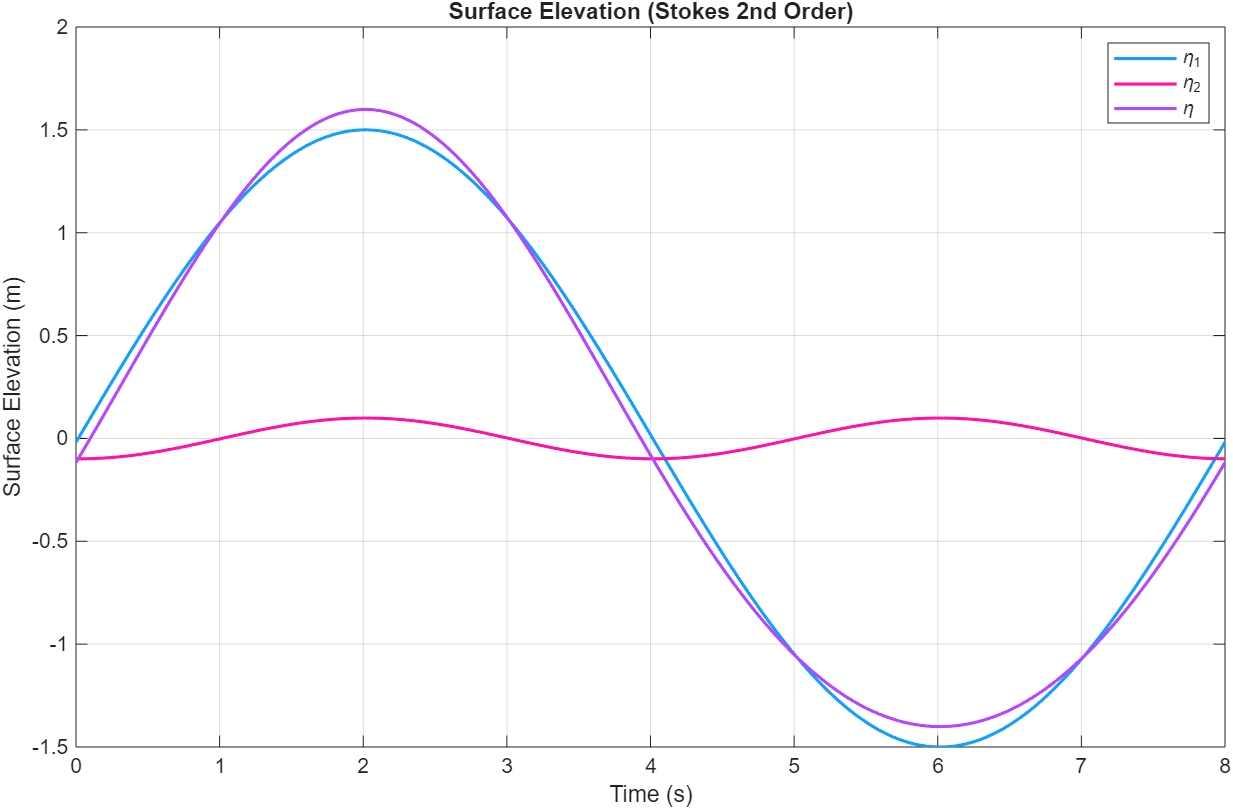
\includegraphics[width=0.6\textwidth]{CE591HW1-Q1a.png}
    \caption{\small Surface elevation plot for Stokes' second-order wave theory.}
    \label{fig:plot2a}
\end{figure}
\vspace{0.3cm}

The surface elevation plot illustrates Stokes’ second-order wave theory, combining a first-order sinusoidal wave ($\eta_1$) and a smaller second-order correction ($\eta_2$). The linear term ($\eta_1$) dominates the wave shape, while $\eta_2$ introduces asymmetry by sharpening crests and flattening troughs. At crests, $\eta_2$ adds to $\eta_1$, increasing peak height. At troughs, $\eta_2$ opposes $\eta_1$, reducing depth. The second-order term remains minor caused by the weak non-linearity. This confirms Stokes’ theory accurately models wave steepening under the given conditions.
\vspace{0.3cm}

\textbf{(b)} Make a plot of the vertical variation of horizontal (\(u\)) and vertical (\(w\)) particle velocities
\begin{figure}[H]
    \centering
    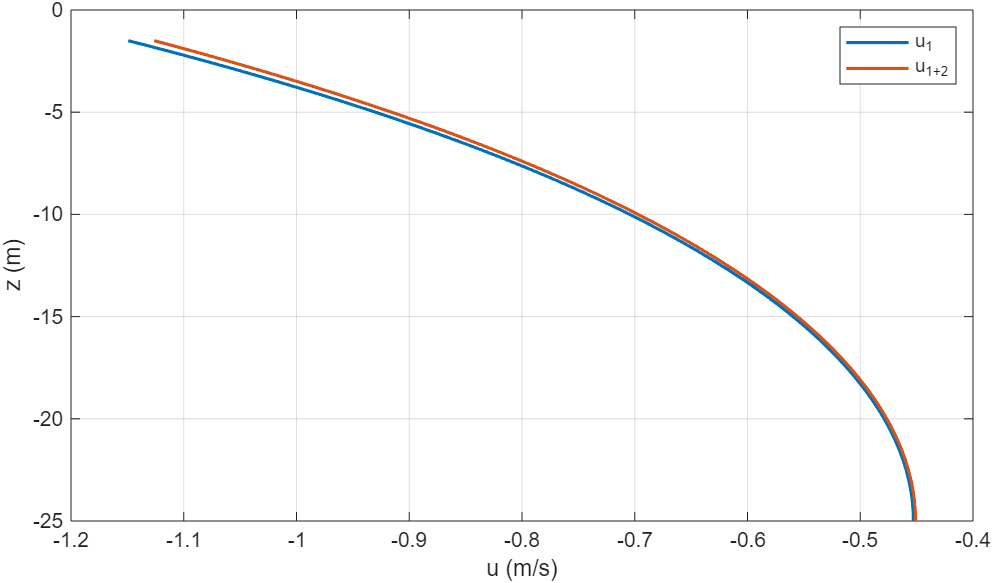
\includegraphics[width=0.8\textwidth]{CE591HW1-Q1b.png}
    \caption{\small Velocity profiles for Stokes' second-order wave theory.}
    \label{fig:plot2b}
\end{figure}
\vspace{0.3cm}

The velocity profiles illustrate the decay of horizontal (\(u\)) and vertical (\(w\)) velocities with depth. At \(t = 0\), the vertical velocity (\(w\)) peaks near the surface and diminishes to zero at the seabed, aligning with linear theory due to the cancellation of second-order terms (\(\sin(2\theta) = 0\)). The horizontal velocity (\(u\)) exhibits a slight non-zero value near the surface in Stokes' theory, exceeding the linear prediction due to second-order corrections. Both components weaken with depth, consistent with theoretical behavior. The results validate Stokes' framework in capturing depth-dependent velocity trends under the given conditions.  
\vspace{0.3cm}

\textbf{(c)} Repeat the calculations in Part (b), changing the water depth as \( h = 20 \, \text{m} \) and \( h = 30 \, \text{m} \). Compare your results with your results from Part (b).
\vspace{0.3cm}


Changing the water depth to \( h = 20 \, \text{m} \) and \( h = 30 \, \text{m} \) alters the velocity profiles:  

\begin{itemize}  
    \item {Shallower depth (\( h = 20 \, \text{m} \))}: Increased bottom influence causes the horizontal velocity to intensify near the surface due to energy concentration, while vertical velocity exhibits more rapid decrease with depth as bottom boundary effects become more dominant.\( u \). 
    \begin{figure}[H]
        \centering
        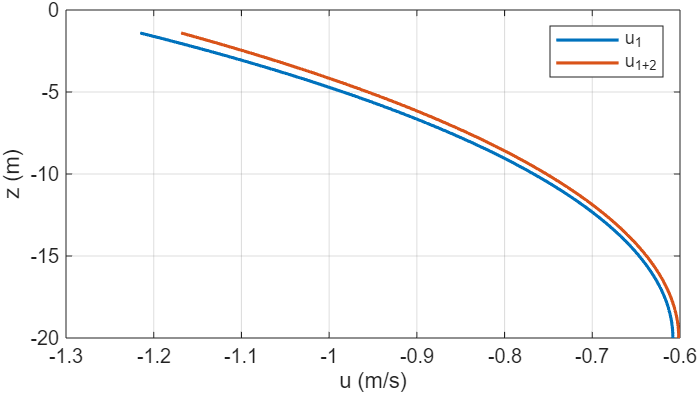
\includegraphics[width=0.8\textwidth]{CE591HW1-Q1c1.png}
        \caption{\small Velocity profiles for h = 20 m.}
        \label{fig:plot2c_1}
    \end{figure} 
    \item {Deeper depth (\( h = 30 \, \text{m} \))}: Bottom inffluence decreases with increased depth. The horizontal velocity weakens near the surface, while the vertical velocity decays more gradually with depth. 
    \begin{figure}[H]
        \centering
        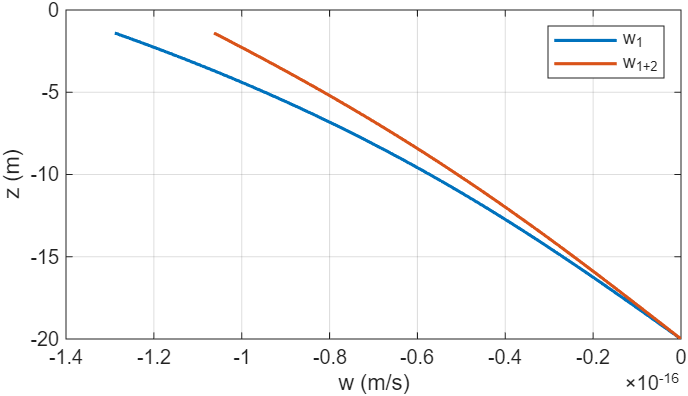
\includegraphics[width=0.8\textwidth]{CE591HW1-Q1c2.png}
        \caption{\small Velocity profiles for h = 30 m.}
        \label{fig:plot2c_2}
    \end{figure} 
\end{itemize}  

\textbf{(d)} Repeat the calculations in Part (b), changing the water depth as \( h = 20 \, \text{m} \) and \( h = 30 \, \text{m} \). Compare your results with your results from Part (b).
\vspace{0.3cm}

\end{document}